\section{FlexUlysses}\label{sec:system_design}


\subsection{Preliminary: Ulysses Sequence Parallelism}

In the Ulysses approach, a sequence $\mathbf{x}$ of length $L$ is split along the sequence dimension across $N$ devices. Each device $i \in \{0, \dots, N-1\}$ receives an equal-sized chunk $\mathbf{x}_i$ of length $L/N$. During the forward pass of a layer, each device computes its local Query ($\mathbf{Q}_i$), Key ($\mathbf{K}_i$), and Value ($\mathbf{V}_i$) tensors from its chunk $\mathbf{x}_i$. To compute the full attention scores, the $\mathbf{K}_i$ and $\mathbf{V}_i$ tensors must be shared among all $N$ devices. This is achieved via an \texttt{all-to-all} communication operation. After the \texttt{all-to-all}, each device possesses the complete Key and Value tensors for a subset of attention heads, allowing it to compute its shard of the attention output. Another \texttt{all-to-all} operation is then performed to gather the output, which is passed to subsequent layers.

\subsection{Sequence Sharding for Load Balancing}

% To address the load imbalance caused by highly skewed sequence lengths, a basic idea is to partition original sequences into smaller, more manageable units. By creating smaller, equal-sized chunks, we establish uniform computational and memory footprints, which provides a crucial opportunity for effective load balancing.

Bucketing fails in scenarios like Figure~\ref{fig:motivation}(Middle), where the \emph{maximum} sequence length is not large enough to require sequence parallelism (SP) for memory, yet the batch exhibits severe length skew. In this regime, the iteration time is dominated by the single longest sequence: regardless of how we bucket or pack samples, the DP rank that receives this outlier becomes the straggler.

We note that Ulysses sequence parallelism implements an equal-cost partition of a sequence. In the MLP module, each GPU receives a shard of the same length, resulting in identical computation and memory footprints. In the attention module, Ulysses computes attention at the head level, and the computation for each head is identical. Therefore, using Ulysses naturally equalizes the computation and memory footprint across GPUs, and it is applicable to any attention pattern. Consequently, applying Ulysses to packed sequences can also achieve load balancing, as sequence packing is essentially a specific attention pattern (concatenating multiple causal attentions). This differs from RingAttention, which, despite partitioning the sequence, requires meticulously designed partitioning decisions and scheduling for different attention patterns. This inspired us to repurpose this mechanism as a load-balancing primitive: using Ulysses chunks as scheduling units and allocating them across different devices to balance the workload on each GPU, even when original sequence lengths are highly variable.

\noindent\textbf{Strawman Solution: Greedy Sharding.} The most straightforward approach is to pack all sequences in the batch and then apply Ulysses, which would force load balancing across all GPUs. However, it is impractical for two reasons. First, Ulysses' scalability is capped by the number of attention heads~\cite{ulysses}, limiting the effective degree of parallelism. Second, it incurs substantial communication overhead. While the attention computation for packed sequences scales roughly as $O(\sum_i L_i^2)$, the \texttt{all-to-all} communication volume grows with the total token count, increasing the communication-to-computation ratio and leading to a higher GPU idle ratio.

\noindent\textbf{Our Solution: FlexUlysses.}~FlexUlysses addresses this by \emph{adaptively} sharding sequences: instead of sharding every sequence into the same (maximal) number of chunks, it assigns each sequence a sharding degree based on its length and then buckets sequences accordingly. This brings two advantages. First, most sequences do not need to be sharded or only require light sharding to achieve near-optimal load balancing, without incurring communication overhead for the entire batch. Second, since sequences with different SP degrees are processed by different device groups, the \texttt{all-to-all} communication and attention computation are independent across sequences (and across different device groups), which enables pipelining and overlapping communication with computation to reduce idle time (bubbles).

\noindent\textbf{Key Challenges.}~However, this hybrid approach introduces two significant implementation challenges. First, the search space is prohibitively large. Finding an optimal configuration requires solving a two-level combinatorial problem: (a) \textit{Sharding Degree Selection}, which chooses a sharding degree for each of the sequences, yielding a search space that grows exponentially with batch size; (b) \textit{Device Group Placement}, which assigns a concrete GPU group to each sharded sequence. The latter is a constrained combinatorial optimization problem that is intractable to solve exactly in practice, because placements across sequences are coupled and must jointly satisfy per-GPU resource limits. 

Second, the resulting configuration creates a complex co-scheduling problem for computation and communication, which breaks the conventional SPMD paradigm. Each sequence is partitioned into multiple chunks and mapped to different device groups. Chunks on the same GPU may belong to different sequences and thus require different \texttt{all-to-all} groups for communication. These groups may overlap, and an incorrect execution order can lead to deadlocks. Moreover, since \texttt{all-to-all} operations are collective and require synchronization, a naive implementation that serializes the communication for each group would introduce significant GPU idle time (bubbles), diminishing the benefits of FlexUlysses. Scheduling the computation and communication of these chunks to maximize GPU utilization is a non-trivial problem. Therefore, a sophisticated scheduling mechanism is required to manage these diverse computation and communication patterns efficiently.

\subsection{Planning and Scheduling for Load Balancing}

We design a two-level planning and scheduling mechanism to address these challenges. It first determines per-sequence sharding degrees and device groups. Then it orchestrates the Ulysses execution order for the assigned sharded sequences on each GPU. % Importantly, we must avoid deadlocks: a GPU may need to participate in multiple collectives of different group sizes, and issuing collectives in inconsistent orders across ranks can deadlock. We address this by (i) restricting device groups to a hierarchical (laminar) family, and (ii) enforcing a \emph{highest-sharding-first} schedule (largest group first). Besides guaranteeing progress, these constraints also create a regular structure that enables communication--computation overlap (Fig.~\ref{fig:comm_overlap}).

\noindent\textbf{Shard Planning.}~Given a global batch, the single controller collects lightweight metadata and outputs a sharding plan. For each sequence $i$ with length $h_i$, we choose a sharding degree $p_i \in \{1,2,4,\dots,p_{\max}\}$ and assign it to a device group $G_i$ with $|G_i| = p_i$. We pre-instantiate a \emph{hierarchical} set of candidate device groups for all admissible degrees: for each degree $p$, the groups form a partition of GPUs (disjoint and covering), and partitions are nested across degrees (a $p$-group is the union of two $p/2$-groups). For example, on 8 GPUs, the admissible groups include $[0\text{-}7]$ for $p{=}8$, $[0\text{-}3]$ and $[4\text{-}7]$ for $p{=}4$, and $[0,1]$, $[2,3]$, $[4,5]$, $[6,7]$ for $p{=}2$. This hierarchy ensures that any two groups are either disjoint or one contains the other, which enables a simple deadlock-free schedule. In practice, we decouple grouping from placement by first instantiating all admissible groups, then assigning sequences to groups using a lightweight greedy heuristic (Appendix~\ref{appendix:placement}).


\begin{algorithm}[!t]
    \renewcommand{\algorithmiccomment}[1]{\hfill{\color{red}\footnotesize$\vartriangleright$~\textit{#1}}}
    \caption{FlexUlysses Forward Attention Execution.}
    \label{alg:flexulysses_step}
    \begin{algorithmic}[1]
        \Require packed sequence groups $\mathcal{Q}$,$\{(p(SG),G(SG))\}_{SG\in\mathcal{Q}}$
        \Require global HSF-ordered list $\mathcal{O}$ over $\{SG\in\mathcal{Q}:p(SG)>1\}$
        \Statex \textbf{Worker rank $k$ (execution)}
        \State $\mathcal{O}_k \gets [SG\in\mathcal{O}\mid k\in G(SG)]$ \Comment{ordered subsequence}
        \State $\mathcal{U}_k \gets [SG\in\mathcal{Q}\mid k\in G(SG)\wedge p(SG)=1]$ \Comment{no collectives}
        \If{$\mathcal{O}_k\neq \emptyset$} \State launch \texttt{all2all1}($\mathcal{O}_k[1]$) asynchronously \Comment{comm stream} \EndIf
        \State $\Call{RunUnsharded}{\mathcal{U}_k}$ \Comment{hide \texttt{all2all1}}
        \For{$t=1$ \textbf{to} $|\mathcal{O}_k|$}
            \State $SG \gets \mathcal{O}_k[t]$
            \State wait \texttt{all2all1}($SG$)
            \If{$t<|\mathcal{O}_k|$} \State launch \texttt{all2all1}($\mathcal{O}_k[t{+}1]$) asynchronously \Comment{issued at compute start} \EndIf
            \State compute attention($SG$)
            \State launch \texttt{all2all2}($SG$) asynchronously \Comment{comm stream}
        \EndFor
    \end{algorithmic}
\end{algorithm}

\noindent\textbf{Highest-Sharding-First Execution.} Collective primitives are order-sensitive: for a given communicator, all ranks must issue collectives in the same order; otherwise, execution can hang. With multiple sharding degrees, a GPU can participate in multiple (nested) device groups, and a naive, per-rank execution order can deadlock even when groups are hierarchical. For example, on 4 GPUs, consider a 4-way group $G_4{=}\{0,1,2,3\}$ and a nested 2-way group $G_2{=}\{0,1\}$. If rank 0 enters an \texttt{all2all} on $G_2$ while ranks 1--3 enter an \texttt{all2all} on $G_4$, then rank 0 waits for rank 1 to join $G_2$, while rank 1 waits for rank 0 to join $G_4$, forming a cyclic wait.

FlexUlysses avoids deadlocks by combining hierarchical device groups with a highest-sharding-first (HSF) schedule. HSF then enforces a consistent global order across all ranks: each GPU always executes collectives for larger degrees before smaller ones (e.g., $p{=}8 \rightarrow 4 \rightarrow 2$), and within the same $(p, G)$, it follows a consistent order so the collective call sequence matches across ranks. As a result, a GPU never interleaves collectives from multiple device groups at the same time. With HSF, any rank that belongs to both $G_4$ and $G_2$ must enter $G_4$ collectives before $G_2$ collectives, preventing the cyclic wait.

\noindent\textbf{Vision Tower Balancing.}~Unlike the LLM backbone, the vision tower is naturally parallelizable across images/frames. Vision encoders typically process images independently by stacking them along the batch dimension, and video frames are sampled and processed with intra-frame attention, making computation independent across frames. As a result, vision-tower compute and memory scale near-linearly with the number of images or frames. We leverage this property by distributing images and video frames evenly across GPUs to balance both compute and memory loads.

\subsection{Dynamic Packing and Overlapping}

\noindent\textbf{Dynamic Shard Packing.}~Executing HSF at single-sequence granularity would repeatedly launch small attention kernels and two \texttt{all2all} collectives per sequence, which can incur non-trivial launch overhead and leave little room to hide communication. We therefore pack sequences assigned to the same device group into \emph{sequence groups} and run Ulysses on each group as a unit. Concretely, within each $(p,G)$ we greedily concatenate \emph{short} sequences (e.g., $h_i \le h_{\text{pack}}$) until the packed token count reaches a cap $H_{\text{pack}}$, while keeping long sequences as singleton groups. This bounded packing trades off between overhead amortization and scheduling flexibility: larger groups reduce kernel/collective launch frequency and create longer compute windows to cover \texttt{all2all}, while the caps prevent a pack from becoming a new straggler and preserve enough groups for pipelining.

\noindent\textbf{Overlapping.}~For a single sequence group, Ulysses induces a strict dependency \texttt{all2all1} $\rightarrow$ \texttt{attn comp}  $\rightarrow$ \texttt{all2all2}. Different sequence groups are independent, so we pipeline them to overlap communication with computation, as illustrated in Fig.~\ref{fig:comm_overlap}. When processing sequence groups under HSF, once $SG_j$ enters attention computation, we immediately launch \texttt{all2all1} of the next group $SG_{j+1}$ on the communication stream. 

\begin{figure}
    \centering
    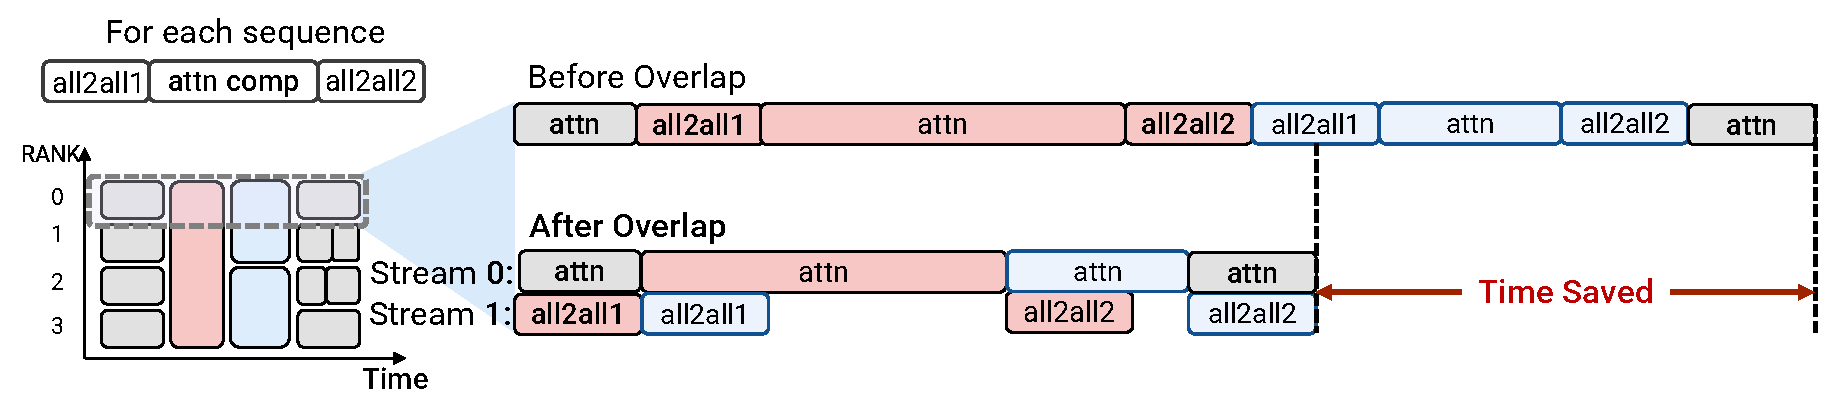
\includegraphics[width=0.95\textwidth]{figures/compute_communication.pdf}
    \caption{Sliced sequence computation pattern of FlexUlysses and communication overlapping strategies.}
    \label{fig:comm_overlap}
\end{figure}


\section{ShadowLoader for the Data-Loading Bottleneck}\label{sec:shadowloader}

To overcome the data loading bottleneck in the hybrid-controller architecture, we design \textbf{ShadowLoader}, a distributed, metadata-driven data-loading system. ShadowLoader consists of four key components: (1) \textbf{Proxy Dataloader}, which resides on the single controller to manage lightweight metadata and dispatch preprocessing tasks; (2) \textbf{Local Preprocessor}, deployed on each worker node to independently handle heavy preprocessing tasks such as video decoding and frame sampling; (3) \textbf{MetaStore}, a registry that maintains the mapping between sample metadata and its physical storage location; and (4) \textbf{Materializer}, instantiated on each worker to fetch the materialized visual tensors from the corresponding Local Preprocessor based on metadata.

% \noindent\textbf{Metadata and FakeTensor.}~
On the single controller, the Proxy Dataloader replaces the standard dataloader. For multimodal data, it only retains lightweight metadata. Specifically, to seamlessly integrate with the existing RL training pipeline, we adopt \texttt{FakeTensor} as a placeholder for visual data. It implements a lazy loading mechanism by storing only metadata, including frame/image count, shape, and file path, and overriding the \texttt{shard} operation to support subsequent partitioning on the first dimension. During training, these \texttt{FakeTensor}s are transferred across different workers according to the batching and load-balancing strategies.

\noindent\textbf{Overall Workflow.}~First, the Proxy Dataloader assigns a unique ID to each data sample and dispatches it to a Local Preprocessor using a simple load-balancing algorithm (e.g., routing to the node with the least load). Upon receiving the task, the Local Preprocessor registers the mapping between the data's metadata and its storage location in the MetaStore. It then executes the preprocessing and caches the materialized visual tensors in its local host memory. Meanwhile, the single controller schedules the RL training loop using the \texttt{FakeTensor}s. When a worker receives a \texttt{FakeTensor} and requires the actual visual data for computation, it invokes its local Materializer. The Materializer queries the MetaStore using the metadata to locate the target preprocessor and fetches the materialized tensors directly from the corresponding Local Preprocessor.

% \noindent\textbf{Distributed Preprocessor Design.}~To address this, we design a distributed dataloader and only transfer \textbf{lightweight metadata of multimodal data} through the single controller. At initialization, a lightweight \textit{Proxy Dataloader} is launched on the master node, and a \textit{Local Preprocessor} is instantiated on each worker node. Both hold only the \textbf{dataset's metadata}, consuming minimal memory. When a batch is requested, the Proxy Dataloader partitions the global batch into shards and distributes these data-loading tasks to the Local Dataloaders. Each Local Dataloader then independently performs the heavy preprocessing tasks—such as decoding, frame sampling, and data augmentation—on its assigned data shard. This distributes both memory and computational loads across the cluster. Once complete, the Local Dataloaders send the metadata of other multimodal data and materialized data of text tensors to the Proxy Dataloader.  Then, the scheduler on the single controller operates on the metadata to determine the optimal data placement across GPUs for vision tower balancing. Finally, the single controller transfer of the metadata of multimodal data to their designated GPUs. Each GPU fetches the desired data on the fly from the corresponding node for load balancing

% Through these mechanisms, ShadowLoader effectively resolves the single-controller bottleneck, enabling large-scale distributed training with larger batch sizes and complex visual data while avoiding CPU OOM and stragglers. 
To further remove data processing from the critical path and minimize overhead, we introduce two additional optimizations to reduce transfer volume and hide latency:

\noindent\textbf{Prefetching and Asynchronous Materialization.}~ShadowLoader overlaps data movement with training by prefetching the metadata for the next step and materializing visual tensors asynchronously on the workers. By launching non-blocking materialization, CPU-side fetching, decoding, and network transfers can be largely hidden behind ongoing GPU computation, substantially reducing bubbles caused by large visual payloads.

\noindent\textbf{FlexUlysses-aware Loading.}~We further co-design ShadowLoader with FlexUlysses by making sharding decisions early and loading only the required data slices. Because the \texttt{FakeTensor} placeholders carry slice-aware metadata, workers can fetch precisely what they need—such as specific frame ranges for videos or required image tensors for multi-image inputs. Aligning this slice-aware materialization with FlexUlysses partition decisions significantly reduces inter-node transfer volume and improves end-to-end throughput.
